%%
% La siguiente plantilla esta basada en el siguiente enlace:
% http://academic.reed.edu/physics/courses/Physics332.s08/reports.html
% La plantilla original puede descargarse de ese sitio
% Se dejo parte del texto original en inglés para ilustar el uso de la plantilla
% Se hicieron algunas modificaciones para ajustar el idioma y otros detalles para 
% completar un reporte técnico breve pero muy puntual
% Modificación Inicial: Marco Aurelio Nuno Maganda - 11/SEP/2014
% 
% Enlace a la documentación del tipo de documento base (revtex4)
% http://mirror.hmc.edu/ctan/macros/latex/contrib/revtex/doc/latex/revtex/source/revtex4-1.pdf
%
% En algunas distribuciones es necesario instalar el paquete texlive-publishers
%
%\documentclass[letterpaper,aps,twocolumn,pre,nofootinbib]{revtex4}
%\documentclass[twocolumn]{article}
\documentclass[conference]{IEEEtran}

\usepackage[spanish]{babel}
\usepackage{amsmath,amssymb,amsfonts,amsthm}
\usepackage{graphicx}
%\usepackage{bbm}
\usepackage[utf8]{inputenc} % Caracteres en Español (Acentos, ñs)
\usepackage{url} % ACENTOS
\usepackage{hyperref} % Referencias
\usepackage{subfig}
\usepackage{lipsum}
\usepackage{balance}


\usepackage{tikz}
\usetikzlibrary{shapes.geometric, arrows}

\tikzstyle{startstop} = [rectangle, rounded corners, minimum width=3cm, minimum height=1cm,text centered, draw=black, fill=red!30]
\tikzstyle{process} = [rectangle, minimum width=3cm, minimum height=1cm, text centered, draw=black, fill=orange!30]
\tikzstyle{decision} = [diamond, minimum width=3cm, minimum height=1cm, text centered, draw=black, fill=green!30]
\tikzstyle{arrow} = [thick,->,>=stealth]

%%%%%%%%%%%%%%%%%%%%%%%%%%%%%%%%%%%%%%%%%%%%%
% PARCHE PARA ELIMINAR LA FECHA DEL DOCUMENTO
% 
\usepackage{etoolbox}
\makeatletter
% \frontmatter@RRAP@format is responsible for the parentheses
\patchcmd{\frontmatter@RRAP@format}{(}{}{}{}
\patchcmd{\frontmatter@RRAP@format}{)}{}{}{}
%\renewcommand\Dated@name{}
\makeatother	
% FIN DEL PARCHE
% 
%%%%%%%%%%%%%%%%%%%%%%%%%%%%%%%%%%%%%%%%%%%%%

%%%%%%%%%%%%%%%%%%%%%%%%%%%%%%%%%%%%%%%%%%%%%
% PARCHE PARA PERMIRIR UTILIZAR BIBLATEX EN ESTA PANTLLA
%\PassOptionsToPackage{square,numbers}{natbib}
%\RequirePackage{natbib}  
%%%%%%%%%%%%%%%%%%%%%%%%%%%%%%%%%%%%%%%%%%%%%

\usepackage[backend=bibtex,sorting=none]{biblatex}
% Estas lineas permiten romper los hipervinculos muy largos !!!!
\setcounter{biburllcpenalty}{7000}
\setcounter{biburlucpenalty}{8000}
\addbibresource{references.bib}

% Actualiza en automático la fecha de las citas de internet a la fecha de la compilación del documento
\usepackage{datetime}
\newdateformat{specialdate}{\twodigit{\THEDAY}-\twodigit{\THEMONTH}-\THEYEAR}
\date{\specialdate\today}

% la sentencia \burl en las citas... 
\usepackage[hyphenbreaks]{breakurl}

\renewcommand\spanishtablename{Tabla}
\renewcommand\spanishfigurename{Figura}

%\usepackage{datetime}
%\newdateformat{specialdate}{\twodigit{\THEDAY}-\twodigit{\THEMONTH}-\THEYEAR}
%\newdateformat{specialdate}{\twodigit{\THEDAY}-\THEYEAR}
%\date{\specialdate\today}


\begin{document}
%%%%%%%%%%%%%%%%%%%%%%%%%%%%%%%%%%%%%%%%%%%%%
% Definitions
%
%
% Define your special symbols here
%
%%%%%%%%%%%%%%%%%%%%%%%%%%%%%%%%%%%%%%%%%%%%%

% use to set width of figures
\newcommand{\breite}{0.9} %  for twocolumn
\newcommand{\RelacionFiguradoscolumnas}{0.9}
\newcommand{\RelacionFiguradoscolumnasPuntoCinco}{0.45}


%%%%%%%%%%%%%%%%%%%%%%%%%%%%%%%%%%%%%%%%%%%%%
% End Definitions
%%%%%%%%%%%%%%%%%%%%%%%%%%%%%%%%%%%%%%%%%%%%%


%Title of paper
\title{Reporte de Laboratorio 1 \\ Salary Calculator}

% Trabajo Individual
\author{\IEEEauthorblockN{Rodriguez Chavez Ana Cecilia\IEEEauthorrefmark{1}}
% En caso de trabajos en equipo, poner a todos los autores en estricto ORDEN ALFABETICO
%\author{\IEEEauthorblockN{Michael Shell\IEEEauthorrefmark{1},
%Homer Simpson\IEEEauthorrefmark{1},
%James Kirk\IEEEauthorrefmark{1}, 
%Montgomery Scott\IEEEauthorrefmark{1} and
%Eldon Tyrell\IEEEauthorrefmark{1}}
\IEEEauthorblockA{\IEEEauthorrefmark{1}Ingeniería en Tecnologías de la Información\\
Universidad Politécnica de Victoria}
}


%\date{}

\maketitle

\begin{abstract} 
\textbf{Este proyecto desarrolla una aplicación interactiva para calcular y visualizar diferentes tipos de salarios en función de horas trabajadas y días de descanso. Utilizando Android y Java, se implementó una interfaz gráfica que permite al usuario ingresar datos como salario, horas trabajadas por semana, días de trabajo y días de vacaciones. La aplicación ajusta automáticamente el salario según el tipo seleccionado, ya sea por hora, diario, semanal, quincenal, semi-mensual, trimestral o anual. Los resultados se presentan en una tabla, mostrando tanto los salarios ajustados como los no ajustados, lo que facilita la comparación. Esta herramienta es útil para empleados y empleadores que deseen entender y gestionar mejor las compensaciones laborales.}
\end{abstract}


%\maketitle must follow title, authors, abstract, \pacs, and \keywords




\section{Introducción}

En este trabajo se presenta el desarrollo de una aplicación gráfica interactiva para el cálculo y visualización de salarios en función de horas trabajadas y días de descanso. La implementación se realiza utilizando Android \cite{anatohipervisor1} y Java \cite{anatohipervisor2}, lo que permite una integración efectiva entre una interfaz de usuario amigable y cálculos dinámicos. El objetivo principal es ofrecer una herramienta que facilite la comprensión de los diferentes tipos de salarios, incluyendo ajustes por vacaciones y días festivos. A través de esta aplicación, los usuarios pueden ingresar datos como salario, horas trabajadas y días de vacaciones, y obtener resultados instantáneos que muestran tanto los salarios ajustados como los no ajustados. Esta aplicación es de particular interés para empleados y empleadores, ya que proporciona una manera clara y accesible de gestionar y entender la compensación laboral.


\section{Desarrollo Experimental}

En este proyecto se desarrolló una aplicación gráfica interactiva para calcular y visualizar salarios en función de las horas trabajadas, días de descanso, y otros factores como vacaciones y días festivos. La aplicación se implementó en Android utilizando Java, lo que permite una integración efectiva entre una interfaz de usuario amigable y cálculos dinámicos.

Inicialmente, se investigaron los conceptos relacionados con el cálculo de salarios, incluyendo el salario base, horas extras, y ajustes por días de vacaciones y festivos\cite{anatohipervisor3}. Este entendimiento permitió diseñar una interfaz gráfica que muestra cómo se comporta el salario en función de las entradas proporcionadas por el usuario\cite{anatohipervisor4}.

El desarrollo de la aplicación se estructuró en varias etapas. Primero, se diseñó la ventana principal utilizando Android Studio, donde se integraron los elementos gráficos necesarios para la interacción del usuario\cite{anatohipervisor5}. Posteriormente, se implementaron los cálculos para determinar el salario total, tanto ajustado como no ajustado\cite{anatohipervisor6}, permitiendo a los usuarios ingresar datos como el salario base, horas trabajadas, y días de vacaciones.

Para la representación gráfica del salario, se utilizaron tablas\cite{anatohipervisor7} que muestran los resultados en diferentes categorías: salarios ajustados y no ajustados. Los cálculos implementados en la aplicación permiten a los usuarios obtener resultados inmediatos\cite{anatohipervisor8}, mejorando la experiencia y la comprensión del proceso de cálculo de salarios.

El código de la aplicación se estructuró de manera modular\cite{anatohipervisor9}, lo que permite la fácil modificación de parámetros como el salario base, las horas trabajadas, y otros ajustes. Esta modularidad también facilita el mantenimiento y la expansión futura del sistema. Se implementaron medidas para asegurar que la visualización\cite{anatohipervisor10} se mantuviera clara y precisa en toda la gama de entradas posibles, proporcionando una experiencia de usuario intuitiva y educativa.

Se realizaron pruebas exhaustivas para verificar la funcionalidad del sistema. Estas pruebas confirmaron que la aplicación proporciona cálculos precisos y consistentes con las normativas laborales. El resultado es una herramienta que ayuda a los usuarios a comprender cómo se determinan sus salarios en función de diferentes variables.

\begin{figure}[h]
\centering
\begin{tikzpicture}[node distance=1.4cm]

\node (start) [startstop] {Inicio};
\node (init) [process, below of=start] {Inicializar SalarioCalculator};
\node (createWidget) [process, below of=init] {Crear widget central y layout};
\node (createInputFields) [process, below of=createWidget] {Crear campos de entrada para datos};
\node (createButton) [process, below of=createInputFields] {Crear botón para calcular salario};
\node (connectButton) [process, below of=createButton] {Conectar botón a calcularSalario};
\node (getInputs) [process, below of=connectButton] {Obtener datos de entrada};
\node (calculateSalary) [process, below of=getInputs] {Calcular salario total};
\node (determineAdjustments) [process, below of=calculateSalary] {Determinar ajustes por vacaciones y días festivos};
\node (displayResults) [process, below of=determineAdjustments] {Mostrar resultados en la interfaz};
\node (end) [startstop, below of=displayResults] {Fin};

\draw [arrow] (start) -- (init);
\draw [arrow] (init) -- (createWidget);
\draw [arrow] (createWidget) -- (createInputFields);
\draw [arrow] (createInputFields) -- (createButton);
\draw [arrow] (createButton) -- (connectButton);
\draw [arrow] (connectButton) -- (getInputs);
\draw [arrow] (getInputs) -- (calculateSalary);
\draw [arrow] (calculateSalary) -- (determineAdjustments);
\draw [arrow] (determineAdjustments) -- (displayResults);
\draw [arrow] (displayResults) -- (end);

\end{tikzpicture}
\caption{Diagrama de flujo del proceso para el cálculo de salarios.}
\label{fig:diagrama_flujo}
\end{figure}




\section*{Resultados}

La aplicación de cálculo de salarios fue desarrollada y probada con éxito, proporcionando resultados precisos y relevantes en función de los datos ingresados por el usuario. A continuación se detallan los principales resultados obtenidos durante la evaluación de la aplicación:


\subsection*{Precisión de los Cálculos}
Se realizaron múltiples pruebas utilizando diferentes combinaciones de datos de entrada, incluyendo variaciones en el salario base, horas trabajadas, y días de vacaciones. Los resultados mostraron que la aplicación calcula correctamente el salario total, tanto ajustado como no ajustado, en concordancia con las normas laborales.

%Agregar fotos de los resultados%

\begin{figure}[h]
\centering
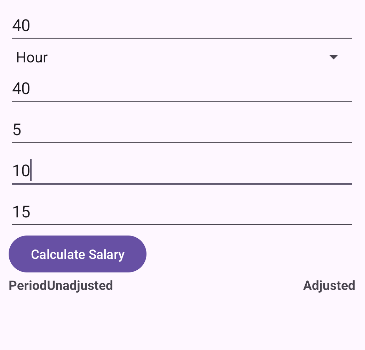
\includegraphics[width=3cm]{1.png}
\caption{Ejemplo de la visualización la interfaz grafica.}
\label{fig:visualizacion_torque}
\end{figure}

\begin{figure}[h]
\centering
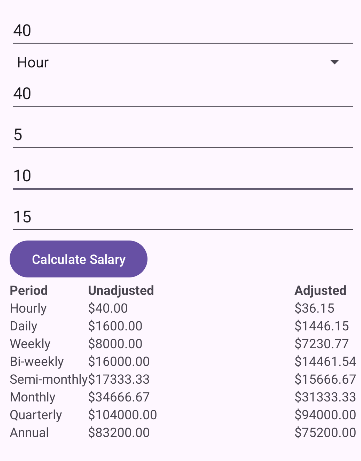
\includegraphics[width=3cm]{2.png}
\caption{Ejemplo de la visualización la interfaz grafica.}
\label{fig:visualizacion_torque}
\end{figure}

\begin{figure}[h]
\centering
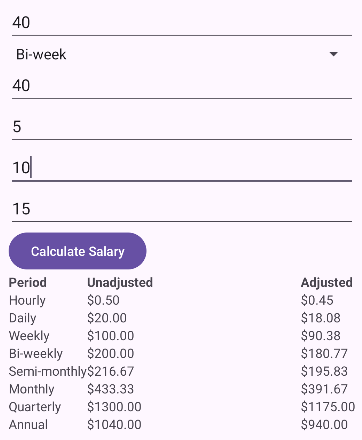
\includegraphics[width=3cm]{3.png}
\caption{Ejemplo de la visualización la interfaz grafica.}
\label{fig:visualizacion_torque}
\end{figure}

\subsection*{Interfaz de Usuario}
La interfaz de usuario fue diseñada para ser intuitiva y fácil de usar. Los usuarios pudieron ingresar datos rápidamente a través de los campos de entrada, y los resultados se mostraron de manera clara y organizada. Se recibieron comentarios positivos sobre la facilidad de navegación y la presentación visual de la información.


\subsection*{Conclusiones}
Los resultados obtenidos confirman que la aplicación es una herramienta efectiva para calcular salarios, proporcionando a los usuarios una forma accesible y precisa de entender cómo sus ingresos se ven afectados por diferentes variables. La combinación de una interfaz amigable y cálculos precisos hace que esta aplicación sea valiosa tanto para empleados como para empleadores en la gestión de salarios.


\addcontentsline{toc}{section}{Referencias} 
\printbibliography
%\balance

\end{document}













